\section{Results and discussion}
\label{sec:resultsAndDiscussion}
In this section, 
we present and discuss results that reveal the effect of fault healing, 
poroelasticity, 
injection rate and more generally injection-time profile, 
on the stability of frictional fault slipping under fluid injection. 

\subsection{Fault healing affects the stability of fault slip significantly}
For a given loading traction of $\tau, \sigma$, 
friction coefficient is set to be $\tau / \sigma$. 
However, 
due to the competing effect of slip rate $V$ and the state variable $\theta$ in (\ref{eq:RSF1}), 
a more healed fault with larger $\theta$ will have a lower initial slip rate $V_{ini}$ under the same loading condition. 
Even though typical slip rate values over a fault long before the nucleation of dynamic events are close to $0$, 
we find that the initial healing (or slip rate) over the fault affects its dynamic behavior significantly under injection. 
Figure~\ref{fig:Vinitial} shows the comparison of slip and friction evolution for $V_{ini}\approx10^{-22}, 10^{-19}, 10^{-16}, 10^{-13}\ \mathrm{m/s}$ under the same flux-controlled injection. 
The flux-control injection in all the cases are kept the same as the baseline case, 
which has a flux of $10^{-4}\ \mathrm{Kg/(m\cdot s)}$ constant in time. 
Materials properties are listed in Table~\ref{tab:elasticBulk} and \ref{tab:fricPropsFault}. 
From figure~\ref{fig:Vinitial} (a) we see that as the fault gets less healed, 
which also means it has higher initial slip rate $V_{ini}$, 
the first dynamic event happens earlier in time, 
and also dynamic events happen more frequently. 
The events expand farther into the fault along $x$ direction. 
Figure~\ref{fig:Vinitial} (b) compares the slip rate at the center of the fault $x = 0$ for the above 4 cases. 
One can see that since the less-healed fault has higher $V_{ini}$, 
under the same injection flux it nucleates the first dynamic event earlier. 
Another thing to keep here is that once a dynamic event nucleates, 
the slip rate is of similar order of $10^{-1}\ \mathrm{m/s}$ for all cases. 
Figure~\ref{fig:Vinitial} (c) plots friction coefficient vs. slip for the above 4 cases. 
We see that the most-healed fault with $V_{ini}=10^{-22}\ \mathrm{m/s}$ has a friction peak of over $0.9$. 
The reason why more-healed faults lead to higher friction peak can be explained by the large gap between their lower initial slip rate and the dynamic slip rate of $0.1\ \mathrm{m/s}$. 
According to (\ref{eq:RSF2}), 
the evolution of $\theta$ happens at a scale of $D_{RS}$, 
and since there is hardly any slip happening before friction reaches its peak, 
$\theta$ is almost still at its initial value. 
Then by this approximation we can write 
\begin{align}
    f_{peak} - f_{ini} &= a \log\left(\frac{V_{dyn}}{V_{ini}}\right) \label{eq:deltF}, 
\end{align}
where $f_{peak}$, $f_{ini}=\tau / \sigma$ are the peak, initial friction; 
$V_{dyn}\approx 0.1\ \mathrm{m/s}$. 

In summary, 
we find that within the typical notion of ``close to zero" initial slip rate, 
the stability of fault slip under fluid injection depends significantly on the initial slip rate, 
and that less healed faults tend to have earlier, more frequent dynamic events that expand farther in space. 


\begin{figure}[htbp]
    \centering
    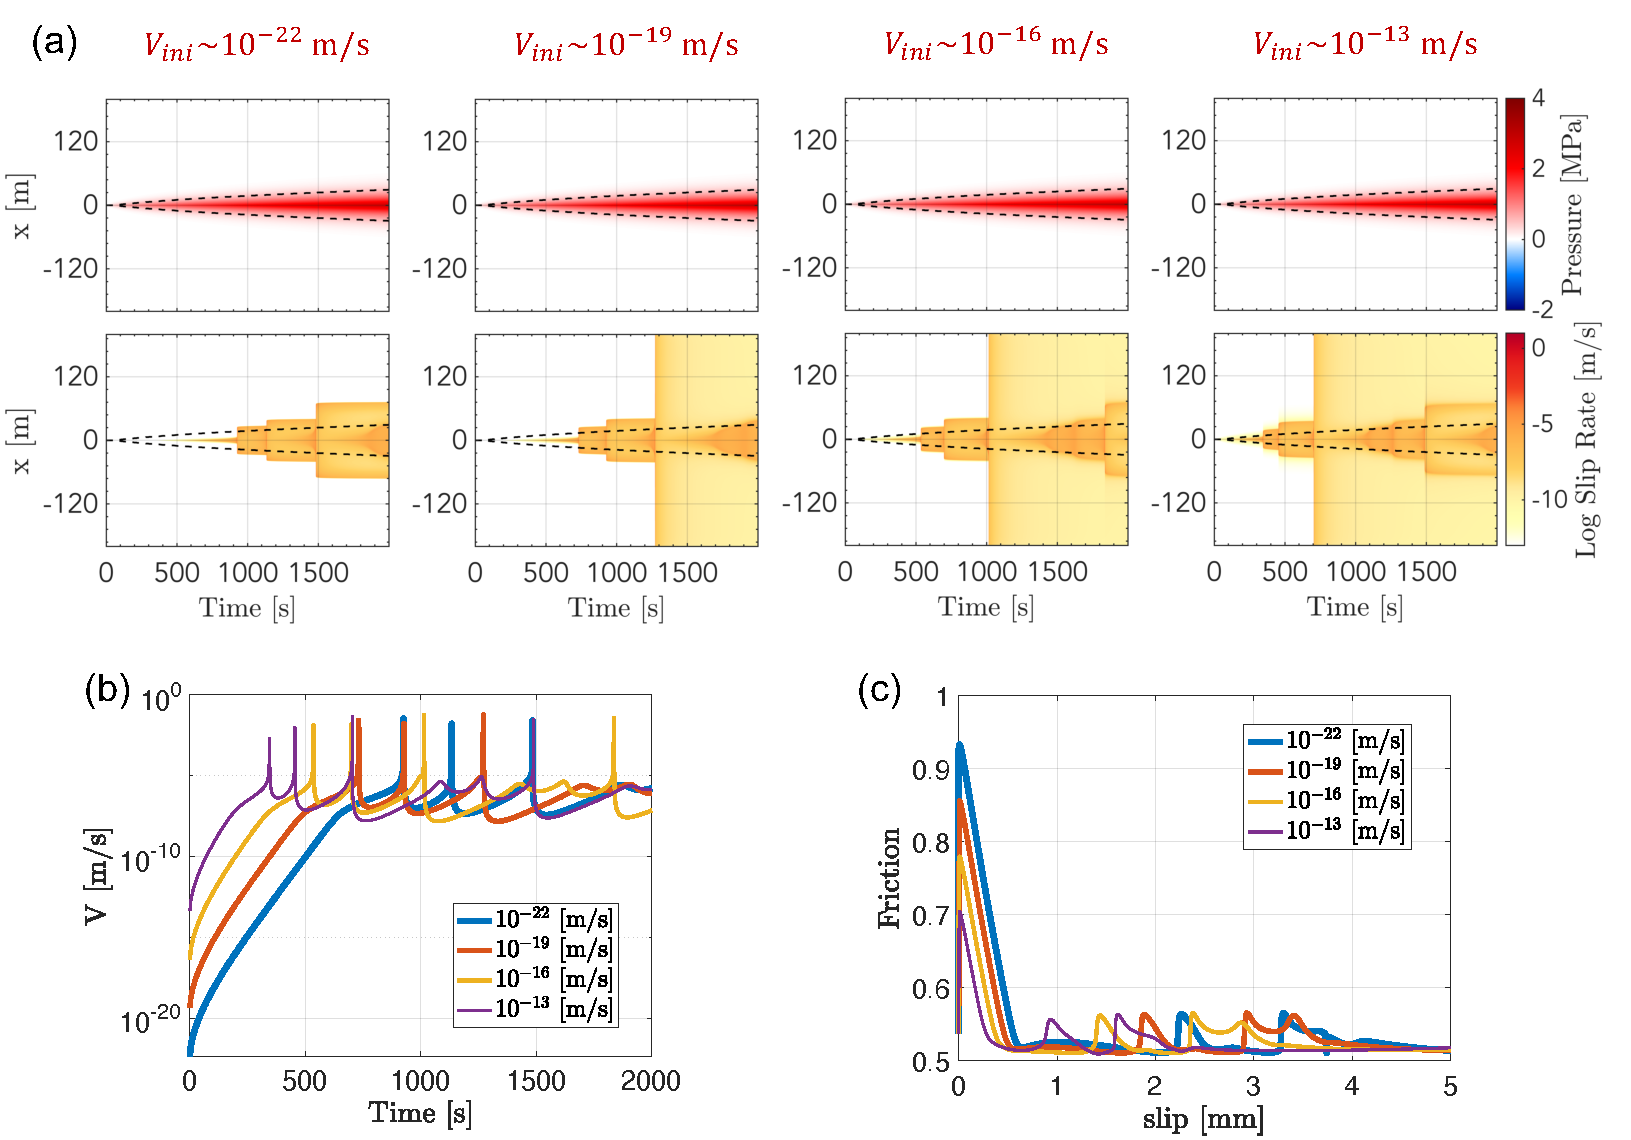
\includegraphics[width=1.0\textwidth]{figures/Vinitial.pdf}
    \caption{Less healed faults with higher initial slip rate tend to be more unstable under the same flux-controlled injection. (a) Comparison of pressure and slip rate vs. time along the fault for $V_{ini}\approx10^{-22}, 10^{-19}, 10^{-16}, 10^{-13}\ \mathrm{m/s}$. 
    (b) Slip rate vs. time at $x = 0\ \mathrm{m}$ for the above 4 cases. 
    (c) Friction vs. slip at $x = 0\ \mathrm{m}$ for the above 4 cases.}
    \label{fig:Vinitial}
\end{figure}

\subsection{Poroelastic effects stablize fault slip under injection}
In (Elias et al., 2022) \cite{Elias_Shengduo_2022}, 
researchers have shown that fault slip gets more unstable as the undrained Poisson's ratio $\nu_u$ decreases and gets closer to Poisson's ratio $\nu$, 
under the same fluid injection. 
And thus it was inferred that poroelasticicty stabilizes fault slip under fluid injection. 
However, 
due to the limitations in the code then, 
researchers were not able to achieve the elastic limit, i.e.,  $\nu_u = \nu$. 
In this study, 
we implement the elastic kernels such that we can indeed simulate cases with $\nu_u = \nu$, 
which equivalently sets $\alpha = 0$, 
and results in the poroelastic equations reduced to elastic equations as given by (\ref{eq:elastic1}, \ref{eq:elastic2}). 
To get a reasonable comparison between elastic and poroelastic cases, 
the governing equations and material properties of the shear layer are kept the same. 
The fluid mobility of the bulk $\kappa$ is kept the same between elastic and poroelastic cases, 
whereas the fluid diffusivity in the bulk is set to either $c=M\kappa$ or $c_{mass}$ given by (\ref{eq:cmass}). 

Since there are two relavant Poisson's ratios, 
namely the undrained $\nu_u$ and the drained $\nu$, 
we consider both elastic cases with Poisson's ratio set to $\nu_u$ and $\nu$, 
and compare them to the poroelastic case with $(\nu, \nu_u)$. 
The material properties are given in Tables~\ref{tab:elasticBulk} and \ref{tab:fricPropsFault}. 

\begin{figure}[htbp]
    \centering
    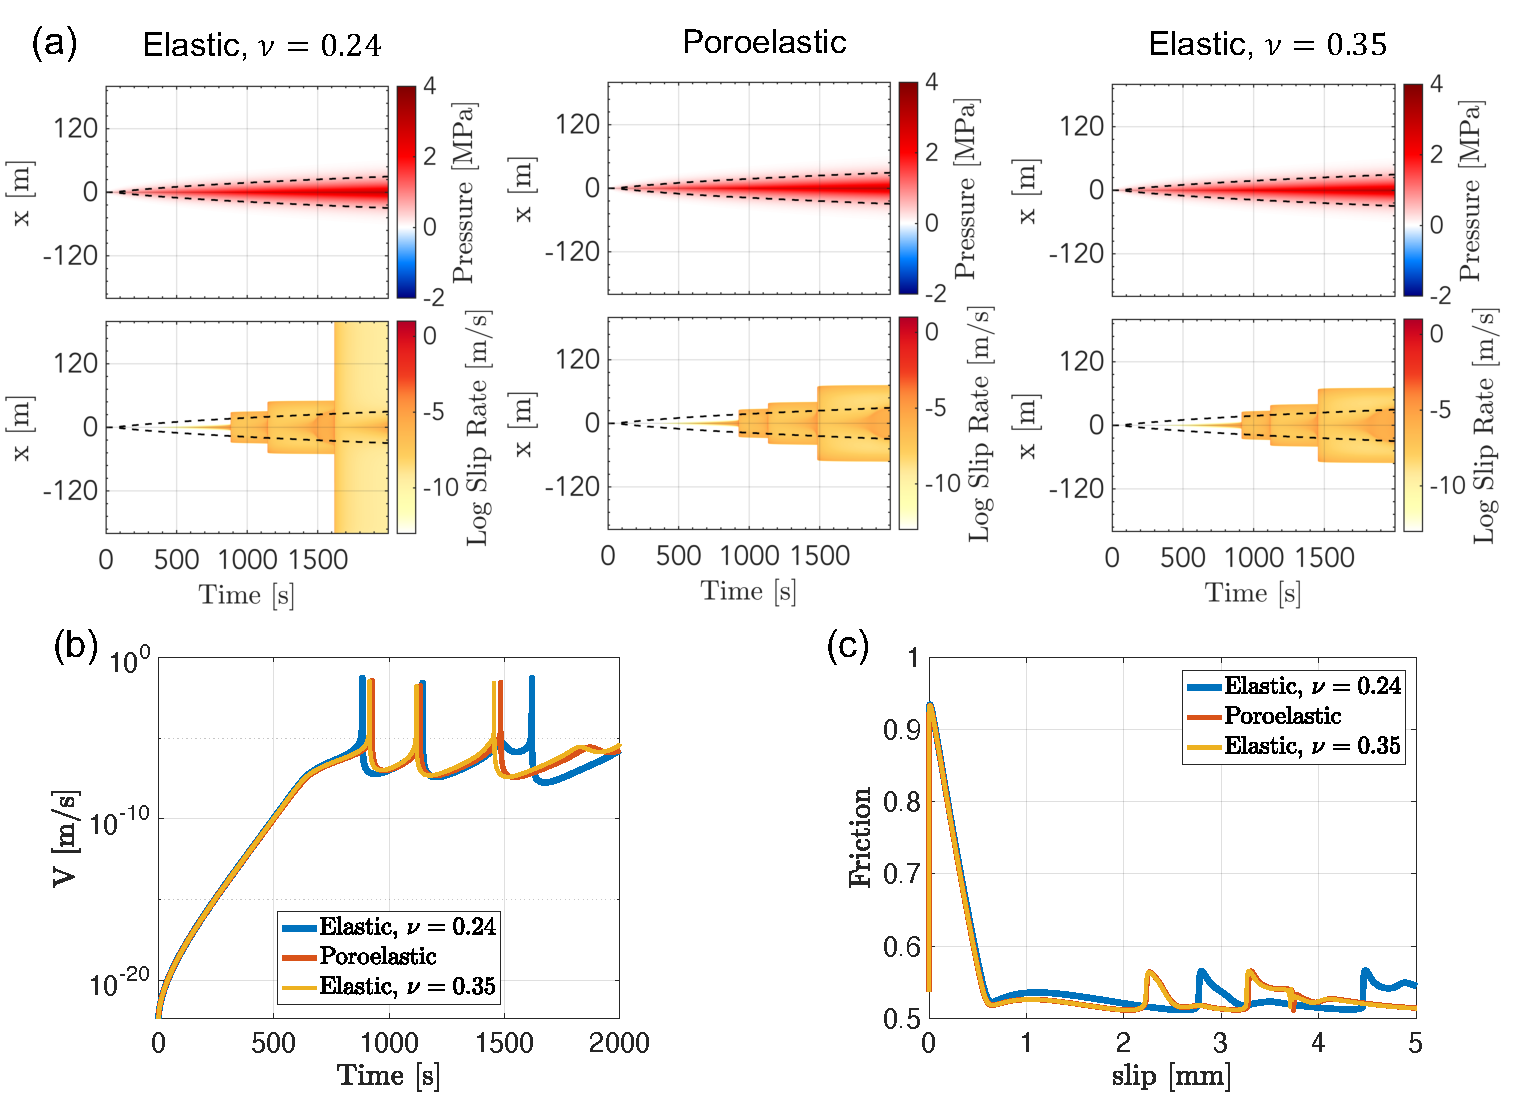
\includegraphics[width=1.0\textwidth]{figures/ElastPoro_c.pdf}
    \caption{Elastic, permeable vs. fully poroelastic bulk when the apparent bulk diffusivity $c$ is kept unchanged. (a) Comparison of average fluid pore pressure change $p_m$ and slip rate $V$ vs. time along the fault for elastic, $\nu = 0.24$, poroelastic ($\nu = 0.24, \nu_u = 0.35$), and elastic $\nu = 0.35$. 
    (b) Slip rate vs. time at $x = 0\ \mathrm{m}$ for the above 3 cases. 
    (c) Friction vs. slip at $x = 0\ \mathrm{m}$ for the above 3 cases.}
    \label{fig:ElastPoroC}
\end{figure}

\begin{figure}[htbp]
    \centering
    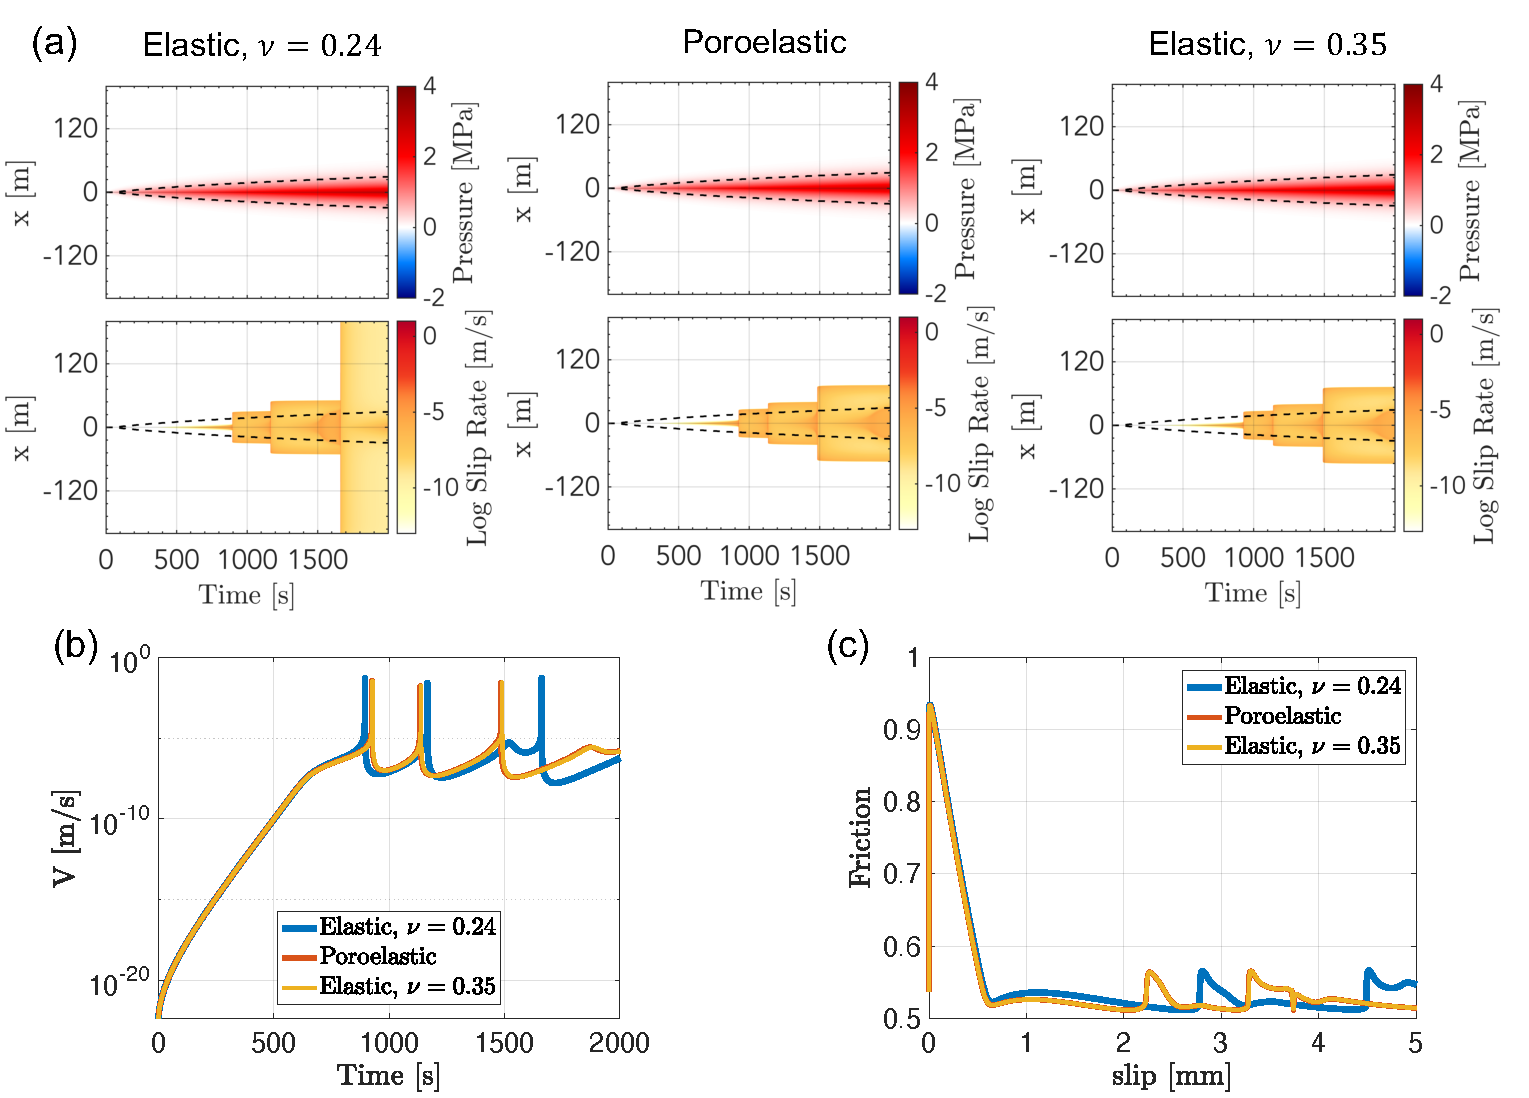
\includegraphics[width=1.0\textwidth]{figures/ElastPoro_cmass.pdf}
    \caption{Elastic, permeable vs. fully poroelastic bulk when the bulk diffusivity for fluid mass content $c_{mass}$ is kept unchanged. (a) Comparison of average fluid pore pressure change $p_m$ and slip rate $V$ vs. time along the fault for elastic, $\nu = 0.24$, poroelastic ($\nu = 0.24, \nu_u = 0.35$), and elastic $\nu = 0.35$. 
    (b) Slip rate vs. time at $x = 0\ \mathrm{m}$ for the above 3 cases. 
    (c) Friction vs. slip at $x = 0\ \mathrm{m}$ for the above 3 cases.}
    \label{fig:ElastPoroCMass}
\end{figure}

Figure~\ref{fig:ElastPoroC} and figure~\ref{fig:ElastPoroCMass} shows the comparison between elastic with drained Poisson's ratio (0.24), 
poroelastic, 
and elastic with undrained Poisson's ratio (0.35). 
The difference between the two figures is that cases in figure~\ref{fig:ElastPoroC} have the same apparent bulk diffusivity $c$, 
while cases in figure~\ref{fig:ElastPoroCMass} have the same $c_{mass}$ as given by (\ref{eq:cmass}). 
The middle columns in the two figures are from the same poroelastic case. 
Both figure~\ref{fig:ElastPoroC} and figure~\ref{fig:ElastPoroCMass} show that, 
under the same flux-control injection, 
the poroelastic case is much more stable than the elastic, permeable case with $\nu = 0.24$, 
and is slightly more stable than the elastic, 
permeable bulk with $\nu = 0.35$. 
This suggests that under such injection and dynamic fault slip condition, 
the poroelastic bulk is close to being undrained. 
Comparing the poroelastic case with elastic, $\nu = 0.35$ case in the two figures, 
we notice that if $c_{mass}$ is kept unchanged, 
using poroelastic bulk or elastic, permeable bulk have almost the same results, 
as shown by figure~\ref{fig:ElastPoroCMass}. 
The slip rate vs. time lines at $x = 0\ \mathrm{m}$ almost overlap perfectly for poroelastic and elastic, $\nu = 0.35$ bulk in figure~\ref{fig:ElastPoroCMass} (b), 
whereas in figure~\ref{fig:ElastPoroC} (b) those two corresponding lines are separating after $1000\ \mathrm{s}$. 
The conclusion is that one can get almost the same results of fault slip under such injection, 
if they replace poroelastic bulk with elastic, 
permeable bulk but keep $c_{mass}$, $\kappa$, $\nu_u$ and $G$ unchanged. 

A simple analysis shows that with realistic material properties of the bulk and the frictional interface, 
the poroelastic bulk would always be close to its undrained limit. 
Denote the characteristic length scale of the pressure front as $D_{ch}$, 
as shown in figure~\ref{fig:CloseTpUndrained}, 
which is usually a fraction of the fault length. 
Denote the propagation speed of the pressure front as $V_{pro}$, 
which is usually a fraction of the shear wave speed of the bulk. 
For any material point adjacent to the fault in the poroelastic bulk, 
the time it is affected by the pressure front is $t_{ch} = D_{ch} / V_{pro}$, 
in which time, 
by 1-D diffusion approximation, 
the pressure on the fault can expand $D_{sp} = \sqrt{t_{ch}c}$ into the bulk. 
For the fluid diffusion in the bulk to be prominent, 
in other words, 
for the bulk to be not almost undrained, 
we would need 
\begin{align}
    D_{sp} &= \sqrt{t_{ch} c_{req}} \approx D_{ch} \notag \\
    c_{req} &\approx D_{ch} V_{pro} \label{eq:estimateC}, 
\end{align}
where $c_{req}$ denotes the required fluid diffusivity, 
and is usually on the order of $10^{3}\ \mathrm{m^2/s}$, 
since $D_{ch}$ is at least on meter level, 
and $V_{pro}$ is on the order of $100\ \mathrm{m/s}$. 
Figure~\ref{fig:CloseTpUndrained} shows the propagation of the pressure front of a case with poroelastic bulk under baseline flux injection, 
in which case the required bulk diffusivity has to be $\approx 1200\ \mathrm{m^2/s}$ to be not almost undrained. 
\begin{figure}[htbp]
    \centering
    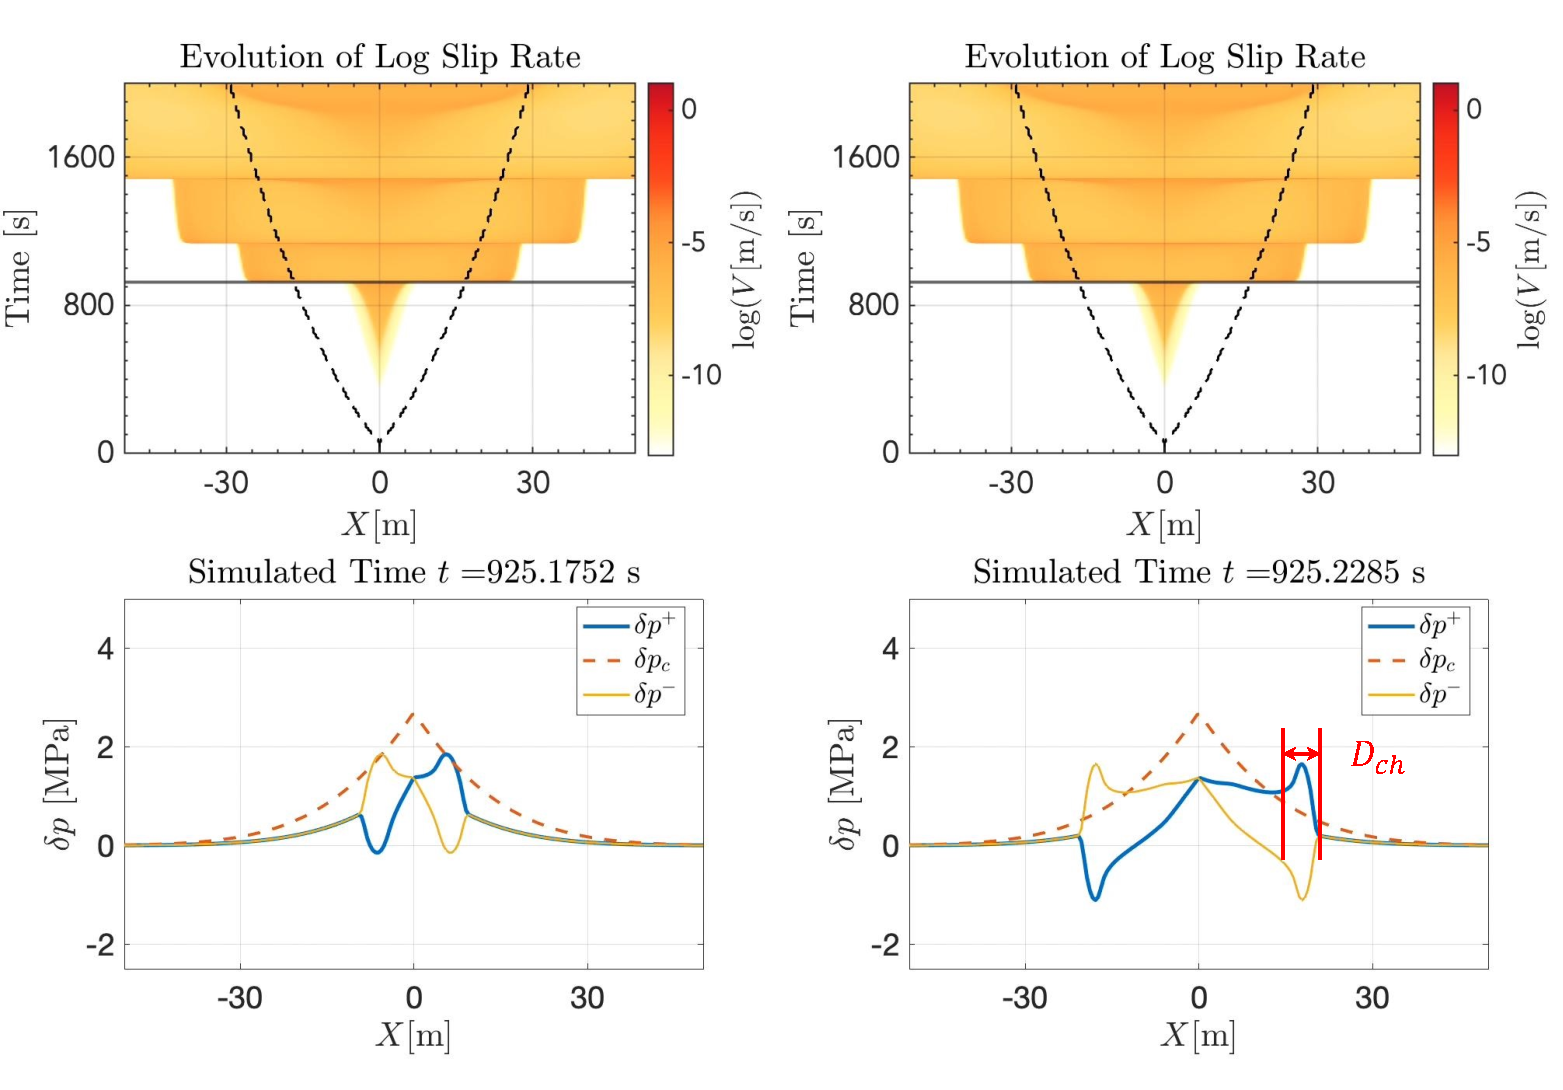
\includegraphics[width=1.0\textwidth]{figures/CloseToUndrained.pdf}
    \caption{The propagation of pressure separation during nucleation of dynamic events due to poroelastic effect. 
    The characteristic length scale of the perturbed pressure front is $D_{ch} \approx 6\ \mathrm{m}$, 
    and from the time difference of the two plots, 
    the propagation speed of the perturbed pressure feature is $V_{pro} \approx 200\ \mathrm{m/s}$
    }
    \label{fig:CloseTpUndrained}
\end{figure}

\subsection{Injection intermittently stabilizes fault slip compared to injection with constant flux} 
Besides studying the effect of poroelasticity vs. elasticity, 
we also look into how the injection flux affects the stability of fault slip. 
First we study for a fixed mass of fluid to be injected, 
whether changing the injection rate (flux) will lead to different fault slip. 
Figure~\ref{fig:fluxPoro} shows the comparison of slip rate vs. time along $x$ for an injection at baseline flux, 
0.75 baseline flux and 0.5 baseline flux. 
The surrounding bulk is poroelastic with properties listed in table~\ref{tab:elasticBulk}. 
The fault properties are listed in table~\ref{tab:fricPropsFault}. 
From figure~\ref{fig:fluxPoro} (a) we see that a larger injection rate leads to earlier, 
more frequent dynamic events but with smaller spatial extent. 
Especially with the smallest injection rate at 0.5 baseline flux, 
even if the dynamic event happens later and less frequently, 
it expands across the entire fault instantly. 
Figure~\ref{fig:fluxPoro} (b) suggests that the dynamic slip rate is similar for all injection rates once a dynamic event happens. 
(c) shows that the friction peak is similar among all three cases because they start from the same initial slip rate, 
and reached similar levels of dynamic slip rate. 

Figure~\ref{fig:fluxElas0.35} in the appendix shows qualitatively similar results for elastic, permeable bulk with undrained Poisson's ratio, 
which confirms that for a given total injected mass of fluid, 
larger injection rate would lead to more frequent but spatially more constrained dynamic slip events. 

\begin{figure}[htbp]
    \centering
    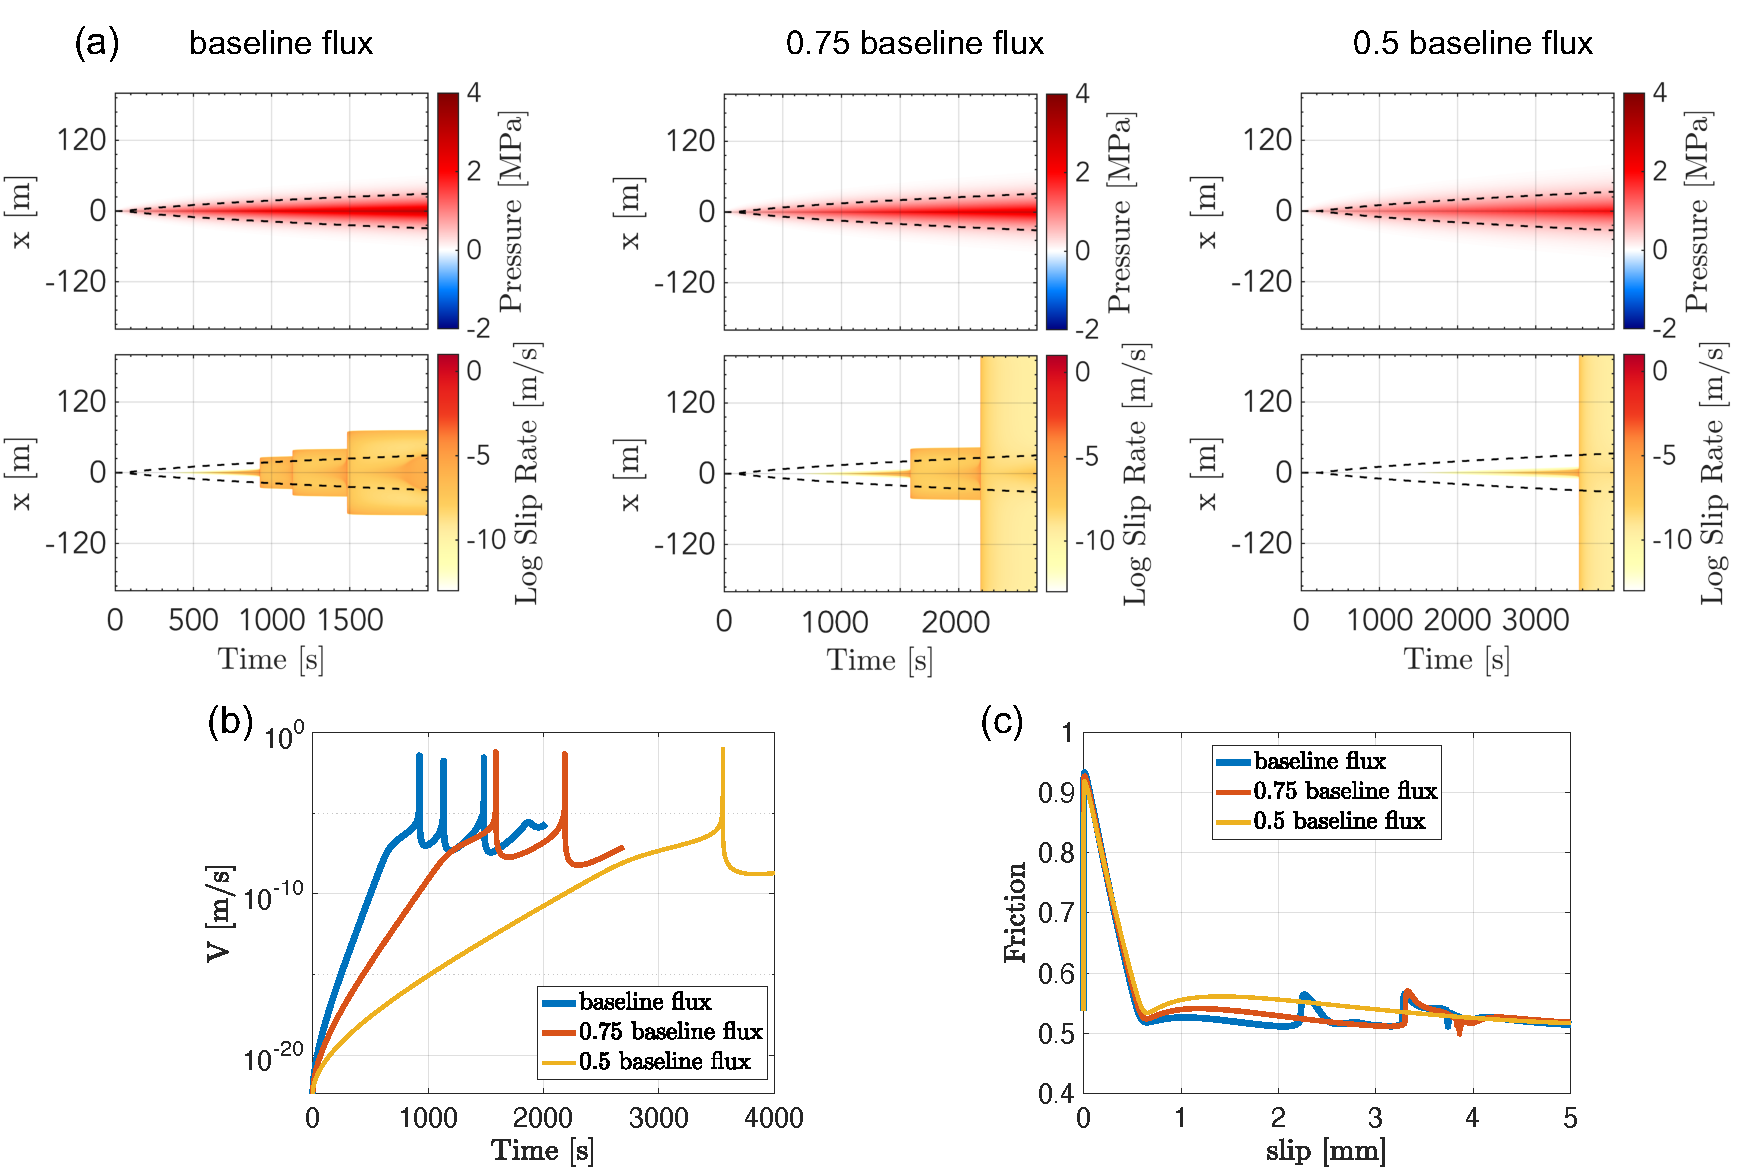
\includegraphics[width=1.0\textwidth]{figures/flux_poro.pdf}
    \caption{The effect of injection rate (flux) on stability of fault slip surrounded by poroelastic bulk. 
    The total injected mass is kept the same for all cases, 
    and thus time is adjusted for different injection rate. 
    Baseline flux is set to be $1.0\times10^{-4}\ \mathrm{Kg / (m \cdot s)}$.
    (a) Pore fluid pressure change and slip vs. time along $x$ for baseline flux, $0.75$ baseline flux and $0.5$ baseline flux. 
    (b) Slip rate vs. time at $x = 0\ \mathrm{m}$ for the above 3 cases. 
    (c) Friction vs. slip at $x = 0\ \mathrm{m}$ for the above 3 cases.}
    \label{fig:fluxPoro}
\end{figure}

Inspired by the fact that a faster injection rate delays the occurence of a spatially wide-spread dynamic event, 
which is usually more destructive, 
we change the injection rate from being constant to being intermittent in time, 
while at the same time also keep the average injection rate and total amount of injected mass the same. 
Figure~\ref{fig:constIntermittent} (b) shows the comparison of slip rate vs. time along the fault between constant and intermittent injection flux. 
The intermittent injection profile results in more frequent dynamic events, 
but none of them expand spatially to the entire fault. 
Figure~\ref{fig:constIntermittent} (c) confirms that in either case the dynamic events have a similar slip rate of $10^{-1}\ \mathrm{m/s}$. 
Since the dynamic events caused by intermittent injection have similar slip rate but more constrained spatial extent, 
it is usually less destructive. 
Figure~\ref{fig:constIntermittent} (d) further confirms that intermittent injection results in smaller total slip. 
This suggests that with some more carefully optimized injection rate-time profile, 
it is possible to achieve more spatially-restricted, 
less destructive dynamic slip events, 
with a given average injection flux as the constraint. 

\begin{figure}[htbp]
    \centering
    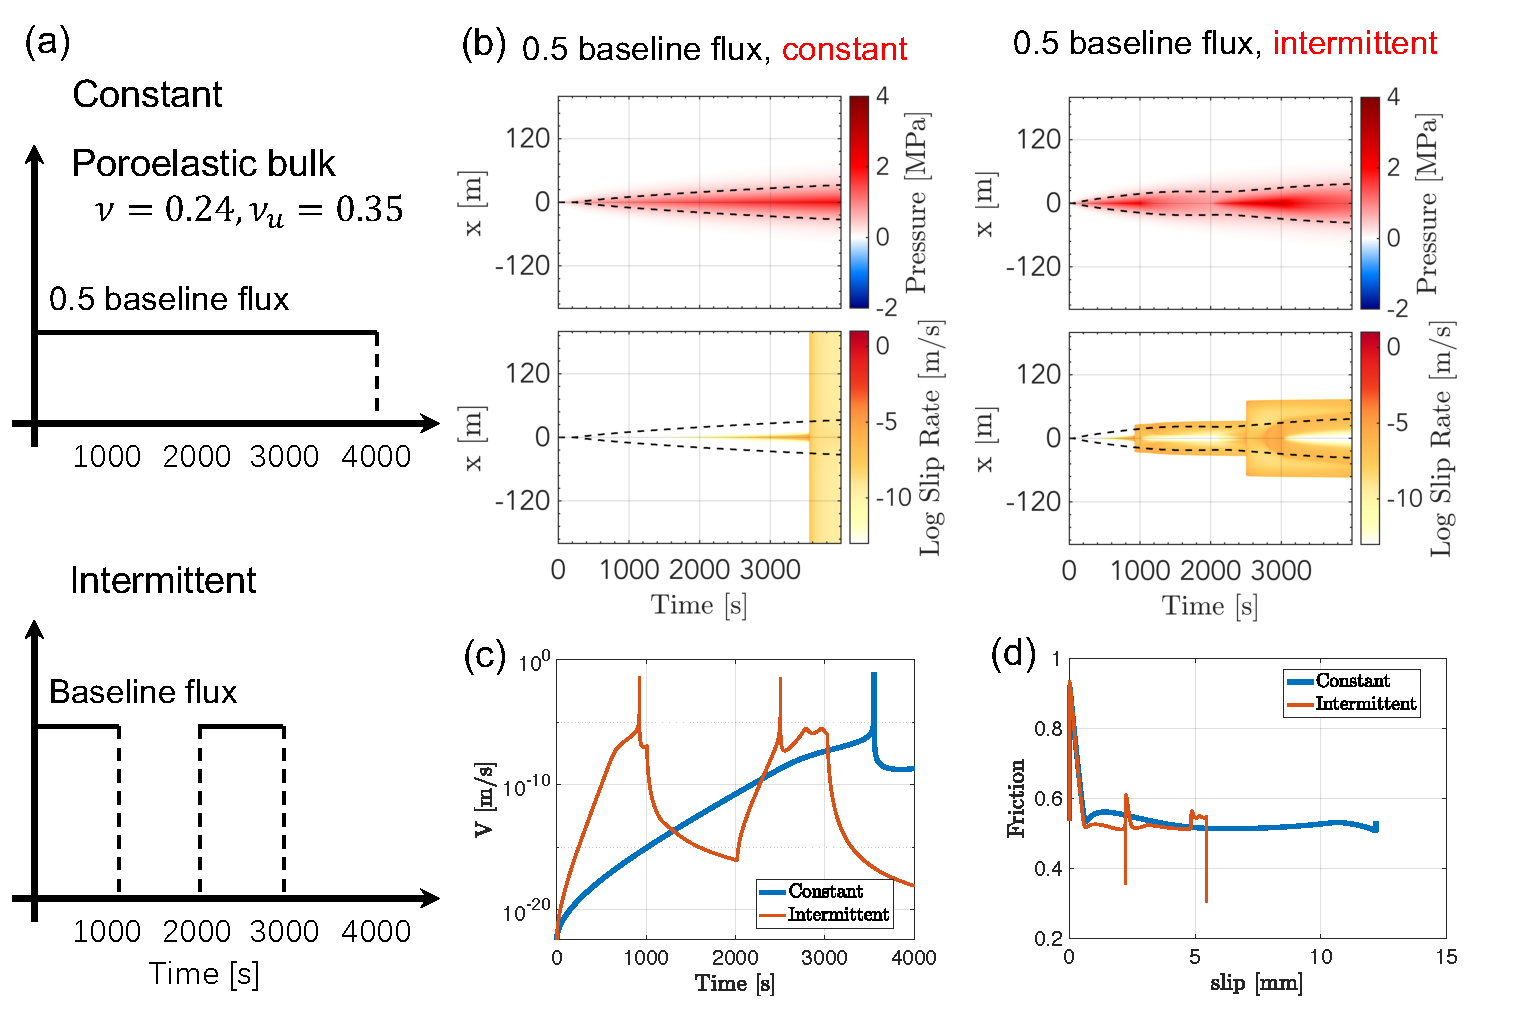
\includegraphics[width=1.0\textwidth]{figures/ConstIntermittent.pdf}
    \caption{Comparison between constant injection rate and intermittent injection rate with poroelastic bulk. 
    (a) Constant and intermittent injection rate as functions of intermittent. 
    (b) Pore fluid pressure change and slip rate vs. time along the fault for constant and intermittent injection rate.
    (c) Slip rate vs. time at $x = 0\ \mathrm{m}$. 
    (d) Friction coefficient vs. slip at $x = 0\ \mathrm{m}$.}
    \label{fig:constIntermittent}
\end{figure}